\documentclass[12pt]{report}
\usepackage[utf8]{inputenc}
\usepackage[english]{babel}
\usepackage{amsmath}
\usepackage{amsfonts}
\usepackage{titlesec}
\usepackage{todonotes}
\usepackage{float}
\usepackage{color}
\usepackage{listings}
\usepackage{lmodern}
\usepackage{graphicx}
\usepackage{bytefield}
\usepackage{tikz}
\usepackage[justification=centering,labelfont={small,bf},font={small,bf}]{caption}
\usepackage[scaled]{beramono} % BitStream Vera font (code)
\usepackage[T1]{fontenc}
\usepackage[a4paper, margin=2.54cm]{geometry}
\usepackage[nottoc,numbib]{tocbibind}

%\renewcommand{\familydefault}{\sfdefault}

\graphicspath{{figures/}}

\usepackage[
style=authoryear,
citestyle=authoryear,
backend=biber,
firstinits=true
]{biblatex}
\DeclareNameAlias{author}{last-first}

\addbibresource{../library.bib}
\DefineBibliographyStrings{english}{%
  references = {References},
}

\lstset{basicstyle=\footnotesize\ttfamily,breaklines=true}

\author{Amy Parent (1303985)}
\title{AHABus \& FCORE:\\Modular Platform for High Altitude Balloon Missions}
\date{April 2017}


% Parameters


\setlength{\baselineskip}{1.5em}
%\linespread{1.3em}

% Title


\makeatletter
\def\maketitle{%
    \vspace*{10em}
	\begin{center}%
	\let \footnote \thanks
        \vskip 5em%
		{\LARGE \textbf{\@title} \par}%
		\vskip 1.5em%
		{\large \@author}%
		\vskip .5em%
		{\normalsize School of Arts, Media and Games\\}%
		\vskip .1em%
		{\normalsize University of Abertay Dundee\\}%
		\vskip .1em%
		{\normalsize Dundee, DD1 1HG, UK}%
	\end{center}
}
\makeatother

\usepackage{datatool}
\usepackage[acronym,toc]{glossaries}
\makeglossaries


\newacronym{fcore}{FCORE}{Flight Computer Operations and Resources Environment}
\newacronym{hab}{HAB}{High-Altitude Balloon}
\newacronym{leo}{LEO}{Low Earth Orbit}
\newacronym{gnss}{GNSS}{Global Navigation Satellite System}
\newacronym{obc}{OBC}{On Board Computer}
\newacronym{ahabus}{AHABus}{Abertay High-Altitude Bus}
\newacronym{fec}{FEC}{Forward Error Correction}
\newacronym{esa}{ESA}{European Space Agency}
\newacronym{i2c}{I\textsuperscript{2}C}{Inter-Integrated Circuit}
\newacronym{spi}{SPI}{Serial Parallel Interface}
\newacronym{ccsds}{CCSDS}{Consultative Committee for Space Data Systems}
\newacronym{ecc}{ECC}{Error-Correction Codes}
\newacronym{rtty}{RTTY}{Radio-Teletype}
\newacronym{aprs}{APRS}{Automatic Packet Reporting System}
\newacronym{pdb}{PDB}{Payload Data Bus}
\newacronym{uart}{UART}{Universal Asynchronous Receiver/Transmitter}

\begin{document}
    
\frontmatter

\begin{titlepage}
\maketitle
\end{titlepage}

\begin{abstract}
\end{abstract}

\tableofcontents
\setlength{\parskip}{1em}

\listoffigures

\listoftables

\printglossary
\printglossary[type=\acronymtype]

\mainmatter

\chapter{Introduction}
\label{ch:introduction}

\newpage
\chapter{Literature Review}
\label{ch:literature-review}

Most \acrshort{hab} missions led by universities, schools or amateur are built 
around commercially available small computers or micro-controller boards:
Redland Green School students used a Raspberry Pi (\cite{rpi2014}) running
python scripts as an \acrfull{obc} for their HAB mission
(\cite{Hinschelwood2015}), while other projects have been ran on AVR
micro-controller based boards like the Arduino Mega
(\cite{AtmelCorporation2015}).

In the United Kingdom, radio licenses do not cover airborne transmission, making
packet radio protocols like AX.25 unusable for HAB missions 
(\cite{ukhasradio2016}). However, the Office of Communications allows the use
of certain \textit{license-exempt} frequencies like the 70cm wavelength band,
provided that the transmission power does not exceed 10mW (\cite{Ofcom2014}).
For this reason, most missions launched from the United Kingdom use the
Radiometrix NTX2 transmitter (\cite{radiometrix2012}). Because of the
constraints, these missions usually transmit their telemetry as text using the
\acrfull{rtty} protocol.

While most \acrshort{hab} projects make use of commercial-off-the-shelf
components, the finished payloads are usually custom, single-purpose designs
that are little, if at all modular. In the design document for the Titan-1 HAB
mission, Bombasaro describes a hardware bus based on tightly coupled sensors
which communicate over two different data buses, SPI and \acrshort{i2c}, and a
custom-made, single-purpose flight software (\cite{Bombasaro2015}).

Because of the risks and cost involved, nano-satellites rely more on modular
designs, allowing each team to work on their module independently. In his paper,
Volstad describes the design of the data bus of the NTNU CubeSat: while the OBC
is a based on a custom made circuit board, it is designed to provide a standard
power interface, as well as access to an \acrshort{i2c} standard bus
(\cite{NXPSemiconductors2014}) to each payload (\cite{Volstad2011}). The
\acrshort{i2c} protocol was chosen because of its low power consumption, and
because if only requires two lines (clock and data). Thomas Clausen describes
in his 2001 paper how a simple packet protocol built on top of \acrshort{i2c}
itself is used for data transfer and error detection in Aalborg University's
CubeSats (\cite{Clausen2001}).

Satellite missions last a lot longer than High-Altitude Balloons' and the
requirements for radio transmissions differ: while satellites can only
communicate when their orbit passes above a ground station and require precise
speed and data volume planning, as described by Sandy Anthunes in his book
(\cite{Antunes2015}), non-floating HAB missions allow for line-of-sight
communications from liftoff to late into the descent of the payload.

There are however some technologies that can be adapted from satellites to be
used in \acrshort{hab} applications. The University of Arizona uses a custom
packet format over 434MHz radio, containing raw binary values for each
instrument's measurements (\cite{Eatchel2002}). The BRITE-Austria CubeSat
mission uses the AX.25 packet radio protocol (used by amateur radio users),
which allows the use of off-the-shelf transmission and reception hardware
rather than custom-made circuits (\cite{Traussnig2007}).

Some nano-satellites use custom telemetry data format, which allows the team
to minimise the volume of data to be sent over radio. The Planetary Society's
Lightsail mission has an uplink connection that allows the ground station
to request specific logs or data. By default, The spacecraft only communicates
a custom beacon containing a summary of the its housekeeping data
(\cite{planetary2016}). Uplink being impractical with the transmission power
limits imposed in the United Kingdom, such a selective telemetry system cannot
be relied upon for \acrshort{hab} missions.

To improve collaboration and allow the deployment of large networks of
satellites, probes and other space vehicles, the Consultative Committee for
Space Data Systems has defined multiple communication standards that for
the different types of networks encountered in spacecrafts.

SpaceWire defines how instruments' data can be accessed by having the OBC
remotely poll their memory (\cite{parkes2005}). A similar system is used to
fetch data from ROM chips over \acrshort{i2c} and could be used to build a
simple data bus.

The \acrshort{ccsds} Space Packet protocol defines a packet format used to
encapsulate application data (from instruments for example) that can be sent
over a ``Space Link'', an analogue of the OSI model's link layer
(\cite{Stallings1987}) using \acrshort{ccsds} frames to encapsulate packets
originating from multiple instruments, ground stations and spacecrafts
(\cite{ccsds2003}).

While \acrshort{hab} applications do not require the level of complexity of
\acrshort{ccsds} protocols — addressing is not needed since the network only
contains two endpoints, communicating in a single direction — some details of
the Space Packet protocol are worth reusing (Forward Error Correction,
different Application IDs for each payload).

\section{Analysis of the Problem}

\newpage
\chapter{Proposed Solution and Methodology}
\label{ch:methodology}

% TODO: add something about:
%       - hardware choices
%       - software choices
%       - language choices
%
%       - overall arch (flight platform, ground segmetn)

The proposed solution for this project is inspired by the bus model that
supports the architecture of most commercial satellites. A standard software
and hardware platform provides common facilities required on all High-Altitude
flights – position tracking, internal data transfers and radio telemetry to the
ground station – allowing payloads (scientific instruments for example) to
only generate data and make it available to the platform.

\begin{figure}[H]
\includegraphics[width=0.35\textwidth]{payloadbus.pdf}
\centering
\caption{Payload bus architecture}
\end{figure}

The platform, or \textit{Payload Bus} is composed of the following components 
hardware and software components:

\begin{description}
    
\item[On Board Computer:] the computer that runs the flight software and
controls the data bus and all communications units (also called
\textit{Bus Controller}).

\item[Flight Software:] the firmware installed on the \textit{OBC}, that
controls the bus and the execution of the mission.

\item[Power Bus:] the hardware interface that provides electrical power to
payloads.

\item[Data Bus:] the hardware interface and software protocol through which
payloads communicate data to the flight computer.

\item[Navigation System:] the hardware (GNSS receiver) and software module used
by the flight software to keep track of the balloon's geographic coordinates and
altitude.

\item[Radio System:] the hardware (transmitter), protocols and software module
used by the \textit{OBC} to transmit collected data and metadata to the
ground station.

\item[Ground Segment:] the software required to record and decode the signal
received from the platform.
    
\end{description}

The following chapter describes the design processes used to develop and
integrate those components into a functioning prototype of the Abertay
High-Altitude Bus (\textit{AHABus}), and the methods used to test the viability
and performance of the design.

\section{Radio Communications Protocol}

This section describes the design process that led to the radio communications
protocol used by the AHABus platform to send payload data and flight metadata
to the ground station. Its role is to ensure that arbitrary binary data – each
payload can use their own data format – as stably and reliably as possible. As
discussed in the following subsections, the design and implementation choice
were also driven by legal constraints: in the United Kingdom, airborne radio
transmitters are limited in frequency band (70cm wavelength) and power
(transmission power inferior to 10mW).

\subsection{Requirements}
\label{ssec:requirements}

Designing and building a communication protocol that can be relied up was an
important requirement for the rest of the project. Transmitting as much as
possible of a mission's scientific data is primordial in case the platform
is carried too far by winds and cannot be recovered after landing.

From the constraints discussed above, the requirements below were established
for the radio communications system:

\begin{enumerate}
\item provide a system to transmit binary data.% DATA LINK
\item minimise the amount of overhead and bandwidth required.% ALL
\item allow multiple payload's data to be sent on the same link.% PACKET LAYER
\item provide stable transmissions on a low-power link.% FRAME LAYER
\item correct as many transmission-induced data errors as possible.% FRAME LAYER
\item allow ground crew to track the balloon's location over time.% PACKET LAYER
\end{enumerate}

As stated in chapter \ref{ch:literature-review}, the United Kingdom's Office
of Communications restrict what frequencies can be used for airborne
radio transmissions, and how much power the transmissions can be sent at.
Those restrictions constrain what existing protocols can be used to transmit
arbitrary data over radio. This disqualifies existing packet radio protocols
that would have fulfilled most of the requirements, in use in other countries
like AX.25.
% TODO: mention Tx only, no Rx

Most UK-launched High Altitude Balloon missions make use of Radio-Teletype
(\textit{RTTY}) to send ASCII-encoded text. This was considered insufficient
for the purpose of a common platform for two main reasons: First, ASCII does
not handle binary data by default -- only some byte values would be displayed
as ASCII, while the rest would translate to non-printing characters. This leads
to data loss, unless the binary data is encoded in an ASCII-compatible format
like base64, which would require more bandwidth to send a similar amount of
data. Furthermore, ASCII alone does not provide either a way to multiplex data
coming from different payloads, or any kind of error checking or error
correction. This means that such facilities must be built on top of the
plain-text protocol.

RTTY itself functions in the same way as wired UART serial links. It can provide
some level of error checking if the transmission of a parity bit is enabled, but
it does not carry enough information to correct errors. Additionally, RTTY is
purely a link layer, and does not provide any kind of encapsulation necessary
for multiplexing data from different payloads.

\subsection{Protocol Specification}

The AHABus radio protocol was designed to match the requirements for the radio
system as closely as possible. While the specification presented in this section
is the last version, which was implemented in the AHABus prototype, some parts
of the protocol evolved or had to be changed during the prototyping process.
% TODO: Might not be necessary to say that here, given further sections

The protocol was designed in layers, some equivalent to the ones present in the
OSI model (\cite{Stallings1987}). This approach was chosen because it allows
some level of modularity – if a layer proves problematic, it can be swapped
for another with minimal impact on the other layers. Each layer fulfils a
specific purpose:

% TODO: Add some details about simplicity of the network topology

\begin{description}
\item[Link Layer:] The lowest-level layer's purpose is to establish a one-way
binary stream between the two end points of the radio link.

\item[Frame Layer:] The frame layer relies on the Link Layer to transmit its
data units, and provides reliability and error correction to higher-level 
layers.
% TODO: Add vocabulary maybe (ancillary)

\item[Packet Layer:] The packet layer is the highest-level layer. It provides
a way for multiple payloads' data to share bandwidth as well as metadata
transmission.
\end{description}

To avoid possible byte order conflicts between the architectures used on the
flight platform and the ground station, multi-bytes values referred to in the
specification should always be transmitted as big-endian (most significant byte
first).

The design process and specification of each of those three layers is explained
in more details in the following sections.

\subsubsection{Link Layer}
\label{sssec:link-layer}

% TODO: add an introductory sentence?

While RTTY was not considered sufficient to cover fulfil the requirements of
the whole protocol, as shown in section \ref{ssec:requirements}, it fulfils the
simple requirements of the Link Layer: it can be used to send 8-bit bytes, one
by one, over a radio link.

RTTY functions like UART, over radio. Instead of using logical electrical levels
(5V for logical high, 0V for logical low), it uses Audio Frequency Shift Keying
(\textit{AFSK}): two audio tones separated by a frequency shift act as two
logical levels. When nothing is being transmitted, the line is held high. The
start of a byte is signalled by the \textit{start bit} (the line goes low),
followed by the eight \textit{data bits}, and one or two \textit{stop bits} (the
line is held high). After a byte has been sent, the line is held high again
until the next byte, or the next byte starts immediately.

Other existing protocols exist that can transmit data over radio audio signals,
like DominoEx or Olivia, sometimes with better transmission rates. RTTY was
preferred over them because the ESP8266 board used as OBC in the AHABus
prototype provides hardware support for UART, making it easier to implement and
reliable. Since the link layer is transparent to the frame and packet layers,
RTTY could be swapped for another protocol in the future with no impact on
those.

The valid encoding and decoding of a \acrshort{rtty} signal depends on the
chosen baud rate (the number of times the logical signal changes level). During
tests, the highest baud rate that allowed clear decoding of radio signals at
\SI{10}{mW} power rating was \SI{200}{bps}. Since each byte requires eleven
bits to be sent (one start bit, eight data bits and two stop bits), this
corresponds to a \(\frac{200}{11}=\SI{18.18}{Bps}\) bandwidth.

\subsubsection{Frame Layer}
\label{sssec:frame-layer}

The role of the frame layer is to provide higher-level layers with a reliable
data stream: the Link Layer discussed in section \ref{sssec:link-layer} will
send data bytes one after another, but it does not guarantee that the bytes are
received, or that noise on the channel (in this case, radio waves) have not
damaged the data between transmission and reception. Those are the two main
potential types of issues that the Frame Layer was designed to address.

Preventing complete data loss on a radio channel is only possible to a degree:
the signal-to-noise ratio is limited by multiple factors including transmission
power – limited in the United Kingdom – distance, other neighbouring
transmissions and line-of-sight. Those issues could have been mitigated in part
through solutions that were outside of this project's scope, like antennae
design. While this meant that some data loss could not be prevented, a solution
was required to detect occurrences of data loss, and identify which part of the
data was missing.

Identifying lost sections of an arbitrary stream of bytes without any form of
formatting is not possible: since it is not known in advance what data should
be expected, there is no model to which actual received data can be compared.
For this reason, the AHABus radio protocol was designed as a framed protocol:
the stream of data is divided in chunks of a set number of bytes, encapsulated
in \textit{frames} that contain the a sequence number used to track the position
of the chunk in the data stream.

The AHABus frame design was inspired by other frame-based protocols like the
CCSDS Space Packet/Frame protocol. Each frame is composed of two section: a
header, that contains metadata, and a payload containing the data carried by
that frame.

The only piece of metadata strictly required to be carried in a frame was its
sequence number. The frame format was designed to use a 16-bit integer to
represent the sequence number, as it allowed a large number of frames to be
sent in-between wrap-arounds of the number (when it becomes larger than 65,535).

To ensure that frames can be identified in the future, even if the format were
to evolve, the protocol version number was also added to the header format. At
the time of this writing, the protocol version was 0. If a future frame decoder
were to receive a frame indicating an old protocol version, it could be at
least signalled to the user, if not handled gracefully.

The resulting first version of the frame format is presented in figure
\ref{fig:frame-fmt-orig}.

\begin{figure}[H]
    \begin{center}
    \begin{bytefield}[bitwidth=0.5em]{64}
        \bitheader{0,8,24,40} \\
        \bitbox{8}{version} &
        \bitbox{16}{seq. number} &
        \bitbox{40}{data[253]}
    \end{bytefield}
    \end{center}
    \centering
    \caption{AHABus Frame Format – Version 1}
    \label{fig:frame-fmt-orig}
\end{figure}

This preliminary design proved impossible to work with: while it encapsulates
the required data and metadata, it does not provide any way to identify the
start or the end of a frame in a raw binary stream, which would have rendered
parsing an incoming frame stream impossible.

To solve this issue, a ``start sequence'' was added at the very beginning of
the frame. When parsing frames from a binary stream, the decoder must ignore
bytes until the start sequence (a single byte of value \texttt{0xAA} followed
by a single byte of value \texttt{0x5A}) occurs. Once the frame sequence is
detected, the frame's end is detected once 256 bytes have been received.

\begin{figure}[H]
    \begin{center}
    \begin{bytefield}[bitwidth=0.5em]{64}
        \bitheader{0,8,16,24,40} \\
        \bitbox{8}{\texttt{0xAA}} & \bitbox{8}{\texttt{0x5A}} & \bitbox{8}{version} &
        \bitbox{16}{seq. number} &
        \bitbox{24}{data[251]}
    \end{bytefield}
    \end{center}
    \centering
    \caption{AHABus Frame Format – Version 2}
    \label{fig:frame-fmt-2}
\end{figure}

The second version of the frame format shown in figure \ref{fig:frame-fmt-2}
fulfils one of its two design goals (detection of data loss). However, it does
not provide a way to detect and correct errors due to noise or interferences on
the radio channel.

The error-correction requirement led to the use of a Forward Error Correction
(\textit{FEC}) algorithm. FEC algorithms function by adding some amount of data
\(D\) to each message sent \(M\). In this case, the message includes both the
frame's header and its payload. \(D\) is computed by the encoder. The decoder
uses \(D\) to detect whether errors were introduced anywhere in the received
block \(M+D\), and correct those errors if their number is below the
algorithm's maximum.

% TODO: block diagram of the encoding-decoding chain

For the purpose of this project, Reed-Solomon(255,223) was chosen for multiple
reasons:

\begin{itemize}
    
\item The Reed-Solomon family of algorithms is widespread in its use, notably
in space communications systems – the Voyager probes used Reed-Solomon codes to
encode their images (\cite{Wicker1994}), the Space Data Links frames (devised
by \acrshort{esa} and \acrshort{ccsds}) use a variant of Reed-Solomon to
provide \acrshort{fec} (\cite{EuropeanCooperationforSpaceStandardization2010})
and the SSDV protocol, used in High-Altitude Balloon missions to transmit
low-resolution images, uses RS(255,223) with 256-byte frames (\cite{UKHAS2016}).

\item There were existing, well tested open-source implementation of that
specific variant of the Reed-Solomon encoders and decoders, which meant that
more time could be spent working on other parts of the project.

% TODO: Ask Ian, transparent might not be the right technical term

\item Reed-Solomon codes are transparent: the original data is not modified for
the purposes of error correction. This means that even if too many errors are
present for the \acrshort{fec} decoder to correct, the data can be manually
inspected and some of it can potentially be saved.
    
\end{itemize}

When applied to 8-bit \textit{symbols} (in this project's case, bytes),
Reed-Solomon codes can only handle blocks (Data and Error-Correction Codes) of
a length up to \(2^{8}-1 = 255\) bytes. The chosen variant, \(RS(223,255)\)
works on 223-byte messages, and adds 32 bytes of Error-Correction Codes at the
end to produce 255-byte blocks. This prompted slight changes in the frame
format: each frame being 256-byte long, one byte would not have been covered
by error correction.

The chosen solution was to not include the start sequence as part of the
error-corrected message. Since proper detection of that sequence is required
for the decoder to start parsing a frame, it would have been impossible to apply
\acrshort{fec} to a frame whose frame start sequence is corrupted.

\begin{figure}[H]
    \begin{center}
    \begin{bytefield}[bitwidth=1.8em]{20}
        \bitbox{1}{...} &
        \bitbox{8}{frame} &
        \bitbox{8}{frame} &
        \bitbox{3}{...}
    \end{bytefield}
    \end{center}
    \centering
    \caption{Frame stream with embedded start sequence}
    \label{fig:frame-sync-emb}
\end{figure}

The start sequence design had to be changed to occupy a single frame byte, as
opposed to two bytes in version 2 of the frame format. Using a single byte to
detect the start of a frame was not deemed sufficient, since the probably of
that exact value occurring elsewhere in the binary stream would have been
fairly high. To mitigate this, the third and final version of the frame format
uses a single frame start marker (\texttt{0x5A}) at the beginning of each
frame, and each frame must be preceded by at least one synchronisation byte
(\texttt{0xAA}), inserted in the binary stream as shown in the lower half of 
figure \ref{fig:frame-sync-extra}. The following 223 bytes in the frame
(starting with the protocol version number) are error-corrected, with the
frame's 32 trailing bytes.

\begin{figure}[H]
    \begin{center}
    \begin{bytefield}[bitwidth=1.8em]{20}
        \bitbox{1}{...} &
        \bitbox{1}{\texttt{AA}} &
        \bitbox{8}{frame} &
        \bitbox{1}{\texttt{AA}} &
        \bitbox{8}{frame} &
        \bitbox{1}{...}
    \end{bytefield}
    \end{center}
    \centering
    \caption{Frame stream with external synchronisation byte}
    \label{fig:frame-sync-extra}
\end{figure}

While this approach may seem wasteful since at least one extra byte must be
inserted in between each frame, it is to be noted that the same synchronisation
byte was previously part of each frame's 256 bytes, leading to a smaller amount
of data being encapsulated in each frame.

\begin{figure}[H]
    \begin{center}
    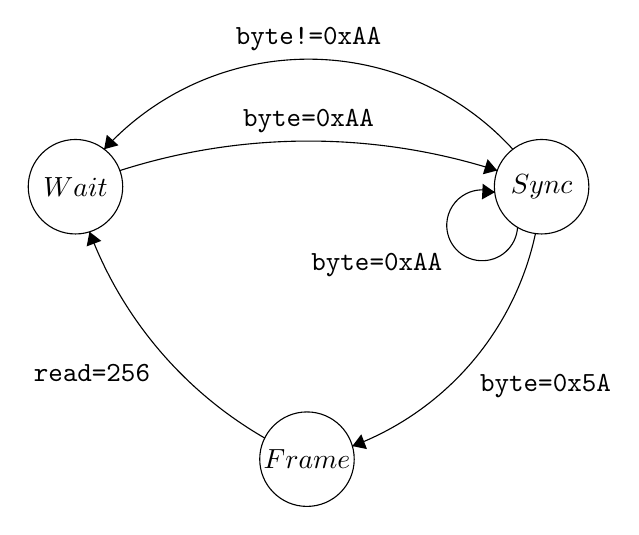
\begin{tikzpicture}[scale=0.2]
    \tikzstyle{every node}+=[inner sep=0pt]
    \draw [black] (23.9,-13.4) circle (3);
    \draw (23.9,-13.4) node {$Wait$};
    \draw [black] (53.5,-13.4) circle (3);
    \draw (53.5,-13.4) node {$Sync$};
    \draw [black] (38.6,-30.7) circle (3);
    \draw (38.6,-30.7) node {$Frame$};
    \draw [black] (26.719,-12.375) arc (107.79277:72.20723:39.209);
    \fill [black] (50.68,-12.37) -- (50.07,-11.65) -- (49.77,-12.61);
    \draw (38.7,-10) node [above] {$\texttt{byte=0xAA}$};
    \draw [black] (53.11,-16.371) arc (-12.09889:-69.37588:18.591);
    \fill [black] (41.48,-29.87) -- (42.41,-30.06) -- (42.05,-29.12);
    \draw (49.56,-26.05) node [right] {$\texttt{byte=0x5A}$};
    \draw [black] (35.918,-29.359) arc (-119.94439:-159.34576:25.489);
    \fill [black] (24.79,-16.26) -- (24.61,-17.19) -- (25.54,-16.84);
    \draw (28.67,-25.22) node [left] {$\texttt{read=256}$};
    \draw [black] (51.972,-15.968) arc (-3.02212:-291.02212:2.25);
    \draw (47.22,-18.39) node [left] {$\texttt{byte=0xAA}$};
    \fill [black] (50.53,-13.75) -- (49.76,-13.21) -- (49.71,-14.21);
    \draw [black] (25.724,-11.023) arc (137.60109:42.39891:17.571);
    \fill [black] (25.72,-11.02) -- (26.63,-10.77) -- (25.89,-10.1);
    \draw (38.7,-4.8) node [above] {$\texttt{byte!=0xAA}$};
    \end{tikzpicture}
    \end{center}
    \centering
    \caption{AHABus Frame Synchronisation State Machine}
    \label{fig:frame-fsm}
\end{figure}

Figure \ref{fig:frame-fsm} presents the finite state machine that
AHABus frame decoders must implement to detect frames in a binary
stream, and figure \ref{fig:frame-fmt-3} the final version of the
AHABus frame format.

% Go to the magic website http://madebyevan.com/fsm/

\begin{figure}[H]
    \begin{bytefield}{16}
        \bitheader{0,7,8,15} \\
        \begin{leftwordgroup}{Header}
            \bitbox{8}{\texttt{0x5A}} & \bitbox{8}{version} \\
            \bitbox{16}{sequence number}
        \end{leftwordgroup} \\
        \begin{leftwordgroup}{Payload}
            \wordbox{2}{data[]}
        \end{leftwordgroup} \\
        \begin{leftwordgroup}{FEC}
            \wordbox{2}{checksum[32]}
        \end{leftwordgroup}
    \end{bytefield}
    \centering
    \caption{AHABus Frame Format - Version 3}
    \label{fig:frame-fmt-3}
\end{figure}
 
%TODO: what's that worth? shouldn't it be at the end

Encapsulating the transmitted data adds overhead. If \(n\) is the size of a
chunk in bytes, and each frame adds \(m\) bytes of metadata, then only a
percentage \(\frac{n}{n+m}\) of the stream contains actual data. For reasons
explained further, the AHABus frames were chosen to be 256-byte
long. As shown previously, each frame also includes.

\subsubsection{Packet Layer}

The Packet Layer relies on the stable data stream provided by the Link and Frame
Layers, and was designed to allow the multiplexing of multiple payload's data as
well as the transmission of ancillary data required for the overall flight
management (platform's GNSS co-ordinates and altitude).

To achieve those goals, the AHABus protocol uses packets similar to frames. Each
packet encapsulates a chunk of data retrieved from a single payload. To that
end, packets were designed to be of variable length, to avoid unnecessary
padding, which would have wasted bandwidth. The data - referred to as the
packet's \textit{payload} – is preceded by the packet's header, which contains
information necessary to attribute the packet's data to a payload, indicate
the length of the packet, and carry the AHABus platform's location and altitude.

This design achieves multiplexing through time division: packets are chunked
and sent in frames one after the other, and can be dispatched to their
respective payload teams once decoded at the ground station. The main issue with
that method is that the protocol itself does not ensure that each payload gets
an even or fair share of the total bandwidth. As discussed in section
\ref{sec:flight-software}, this was solved in the flight software design.

\begin{figure}[H]
    \begin{bytefield}{32}
        \bitheader{0,7,8,15,16,23,24,31} \\
        \begin{leftwordgroup}{Header}
            \bitbox{8}{version} & \bitbox{8}{payload ID} &
            \bitbox{16}{length} \\
            \bitbox{32}{latitude} \\
            \bitbox{32}{longitude} \\
            \bitbox{16}{altitude} & \bitbox[lrt]{16}{}
        \end{leftwordgroup} \\
        \begin{leftwordgroup}{Payload}
            \wordbox[lrb]{3}{data[length]}
        \end{leftwordgroup}
    \end{bytefield}
    \centering
    \caption{AHABus Packet Format - Version 1}
    \label{fig:packet-fmt-1}
\end{figure}

Figure \ref{fig:packet-fmt-1} shows the first and current version of the AHABus
packet format. Like frame discussed in section \ref{sssec:frame-layer}, each
packet carries a version flag which was added to allow backwards compatibility,
were the protocol to evolve in the future.

The encoding of the metadata was chosen based on the physical constraints of
the information:

\begin{itemize}
\item Latitude and Longitudes can be both positive (North, East) or Negative
(South, West). At the equator, \SI{0.0001}{\degree} of longitude maps to
roughly eleven metres\footnotemark , and that distance decreases when moving
towards the poles, which was deemed precise enough for the project's purpose.
To avoid conflicts in floating-point mathematics conventions, and allow packet
encoders to be written for embedded platform without hardware floating point
support, latitude and longitude were designed to be multiplied by 10,000 and
transmitted as 32-bit precision signed integers.

\item Altitude is above zero for the whole mission duration, and cannot exceed
\SI{50000}{\meter}. Since a sub-metre precision is not required, and would
hardly be achievable with civilian GNSS receivers, it is encoded as a 16-bit
precision unsigned integer.

\end{itemize}

\footnotetext{
Earth circumference at the equator: \SI{40e6}{\meter}.
\(D_{\SI{0.0001}{\degree}} = 0.0001\times\frac{40\times{10^6}}{360}=\SI{11.1}{\meter}\)
}

The decision was made during the design process to align packet boundaries with
frame boundaries. This means that every time a new packet is sent through the
radio channel starts at the start of a new frame, instead of being inserted
in the middle of a frame, where the last packet stopped.

This approach leads to a loss in bandwidth: if a packet's length is not a 
multiple of the amount of data that a frame carry, the packet's last frame
will be padded with zeros instead of containing the start of the next packet.
However, it was deemed an acceptable tradeoff because of the issues that
non-aligned (contiguous) packets would present:

\begin{itemize}
\item If a packet's end does not match a frame's end, that frame cannot be
sent until the start of the next packet is known. This meant that the
transmission of most packet's last frames could be delayed for sometimes several
seconds until another packet is processed.

\item In the case where a frame is lost due to channel noise or interferences,
finding the start of the next packet would have been complicated, or required
a synchronisation mechanism similar to the one designed for AHABus frames.
Aligning packets instead makes such a system unnecessary, reducing the packet
header size and the complexity of packet decoders.
\end{itemize}

% TODO: Add diagram explaining aligment

\subsection{Initial Implementation and Testing}

To evaluate the protocol's viability, a full demonstration of an AHABus radio
stack was written. Its main goals were to provide a reference implementation of
a compliant encoder and decoder, validate the protocol's design process, and
test the algorithms used in a controlled environment before integrated testing.

The C language (ISO/IEC 9899:1999 standard) was chosen for the reference
implementation because of its widespread use, and its availability on most
micro-controller and embedded platforms, which would be used as AHABus flight
platforms. To render the code as portable and reusable as possible, care was
taken to limit the dependencies to a subset of the C language standard library,
and avoid use of dynamic memory allocation, which is often inefficient or
unavailable on embedded platforms.

To increase portability and ease of use further, the encoder and decoder read
and write data using user-supplied callback. This allows developers to import
the implementation files and use the library without editing, at the expense of
optimisation.
% TODO: Explain?

\subsubsection{Encoder}

Figure \ref{fig:encoder-flow} illustrate the data flow in the encoder.
In an attempt to use as little memory as possible, no intermediate
representation of the packet is created or stored. Instead, the header and
first chunk of the packet's data is written directly to a frame buffer. Once
the frame is fully constructed, its binary representation is written using the
user-provided callback. The buffer is then cleared, and the process is repeated
until all of the packet's payload has been framed. 

\begin{figure}[H]
\includegraphics[width=0.6\textwidth]{encoder-flow.pdf}
\centering
\caption{Encoder Data Flow}
\label{fig:encoder-flow}
\end{figure}

For testing purposes, a simple program was built that takes in user input,
uses the encoder to package that data and outputs the frame stream to the
UNIX standard output (\texttt{stdout}).

% TODO: more details? how much is required?
% TODO: add reference to appendix with code

\subsubsection{Decoder}

\subsubsection{Initial Testing}

\section{Payload Bus}
\label{sec:payload-bus}

The Payload Bus is the hardware and software interface that is used by the
\acrfull{obc} to communicate with each payload carried on a mission. 

\subsection{Requirements}

\subsection{Initial Prototypes}

Before a protocol was chosen, two different preliminary designs approaches were
prototyped and

\subsubsection


\subsection{Protocol Specification}

\subsection{Arduino Implementation}

\section{Flight Software}
\label{sec:flight-software}

\subsection{Architecture}

\subsection{User Interface}

\section{Ground Segment}
\label{sec:ground-segment}

\subsection{Extracting Raw Binary Stream}

\subsection{Packet}

\section{Testing}
\label{sec:testing}

\subsection{Component Testing}

\subsection{Integrated Testing}

\subsubsection{Day in the life Testing}

\subsubsection{Resilience Testing}

\newpage
\chapter{Results}
\label{ch:results}

\newpage
\chapter{Discussion}
\label{ch:discussion}

\newpage
\chapter{Conclusion}
\label{ch:conclusion}

\printbibliography[heading=bibintoc, title=References]

\end{document}